\documentclass{article}

% Chinese Support using xeCJK
% \usepackage{xeCJK}
% \setCJKmainfont{SimSun}

% Chinese Support using CTeX
\usepackage{ctex}

% Math Support
\usepackage{amsmath}
\usepackage{amsfonts}
\usepackage{amssymb}
\usepackage{wasysym}
\newcommand{\angstrom}{\text{\normalfont\AA}}
\usepackage{fancyhdr}

% Graphics Support
\usepackage{graphicx}
\usepackage{float}

% Reduced page margin
\usepackage{geometry}
\geometry{a4paper,scale=0.8}

\usepackage{caption}
\usepackage{subcaption}

% d and e should be math operators
\newcommand*{\dif}{\mathop{}\!\mathrm{d}}
\newcommand*{\md}{\mathop{}\!\mathrm{d}}
\newcommand*{\me}{\mathrm{e}}

% No indent for each paragraph
% \usepackage{parskip}
% \setlength{\parindent}{0cm}

% Bold style for Greek letters
\usepackage{bm}
\let\Oldmathbf\mathbf
\renewcommand{\mathbf}[1]{\boldsymbol{\Oldmathbf{#1}}}

% More space for dfrac in cell
\usepackage{cellspace}
\setlength{\cellspacetoplimit}{5pt}
\setlength{\cellspacebottomlimit}{5pt}

% SI units
\newcommand{\si}[1]{\  \mathrm{#1}}

% Multi-line author information
\usepackage{authblk}
\author{物理(4+4)1801 \quad  胡喜平 \quad U201811966}
\affil{个人网站 https://hxp.plus/ \quad 电子邮件 hxp201406@gmail.com}

\title{近代物理实验预习笔记——晶体的电光调制}

\pagestyle{fancy}
\fancyhf{}
\lhead{源码地址:https://github.com/hxp-plus/Notes/tree/master/Physics-Experiment}
\rfoot{第 \thepage 页}
\renewcommand{\headrulewidth}{1pt}
\renewcommand{\footrulewidth}{1pt}

\begin{document}

\maketitle\thispagestyle{fancy}

\section{实验内容}

\begin{itemize}
\item 观察电光效应,测量晶体的\textbf{半波电压}。
\item 改变晶体的工作点,观察\textbf{线性调制}、\textbf{倍频失真}、\textbf{非线性调制}。
\item 用1/4波片改变工作点,观察晶体的\textbf{倍频失真}和\textbf{线性调制}。
\end{itemize}

\section{实验原理和注意事项}

\subsection{横向电光调制原理}

下图是晶体横向电光调制装置图,入射光经过起偏器成为平行于x轴的线偏振光,通过电光晶体,$x$分量和$y$分量产生相位差$\delta_1$,通过1/4波片再产生相位差$\delta_2$,最终从平行于$y$轴的检偏器出射。

\begin{figure}[H]
  \centering
  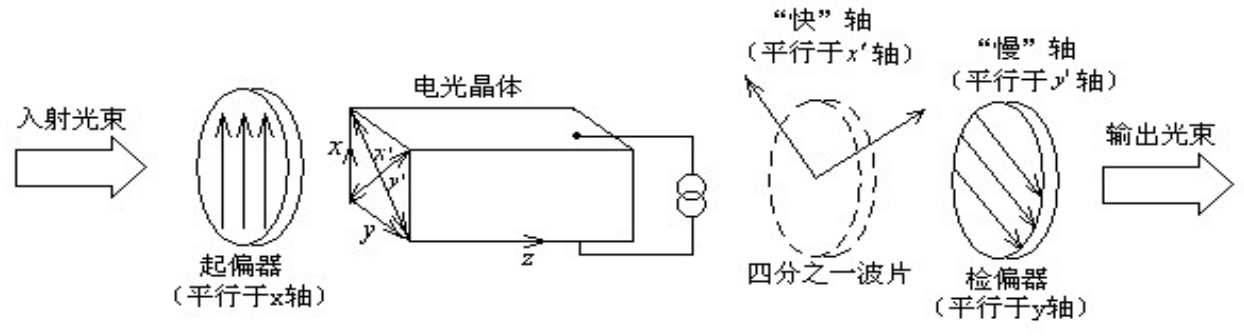
\includegraphics[width=0.9\linewidth]{figures/晶体的横向电光调制}
  \caption{晶体的横向电光调制装置图}
\end{figure}

其中光通过电光晶体产生的相位差$\delta_1$是正比于电光晶体上加的电压的,为

\begin{equation*}
  \begin{aligned}
    \delta = \dfrac{2 \pi}{\lambda} n_0^3 \gamma_{22} V \dfrac{\lambda}{d}  
  \end{aligned}
\end{equation*}

同时,光透过检偏器后透射率为

\begin{equation*}
  \begin{aligned}
    T = \sin^2 \dfrac{\delta_1 + \delta_2}{2} 
  \end{aligned}
\end{equation*}

当晶体两端电压在某一个特定数值的时候,光透过晶体产生$\pi$的相位差,定义这个电压为$V_{\pi}$,则

\begin{equation*}
  \begin{aligned}
    V_{\pi} = \dfrac{\lambda}{2 n_0^3 \gamma_{22}} \left( \dfrac{d}{l}  \right)  
  \end{aligned}
\end{equation*}

则

\begin{equation*}
  \begin{aligned}
    \delta_1 = \pi \dfrac{V}{V_{\pi}} 
  \end{aligned}
\end{equation*}

\subsection{依靠改变直流偏压的电光调制}

如果我们把直流偏压$V_0$和交流调制信号$V_m \sin \omega t$同时加到电光晶体两端,随着交流调制信号的改变,透过率也会改变。

\begin{equation*}
  \begin{aligned}
    T = \sin^2 \dfrac{\delta_1}{2} = \sin^2 \dfrac{\pi}{2 V_{\pi}} \left( V_0 + V_m \sin \omega t \right)  
  \end{aligned}
\end{equation*}

调制信号不失真应当有两个前提:$V_0$设置的静态工作点处,透射率对于晶体两端电压的偏导数是$1$,且$V_m \ll V_0$。原因看下面的图自然很容易就明白。

\begin{figure}[H]
  \centering
  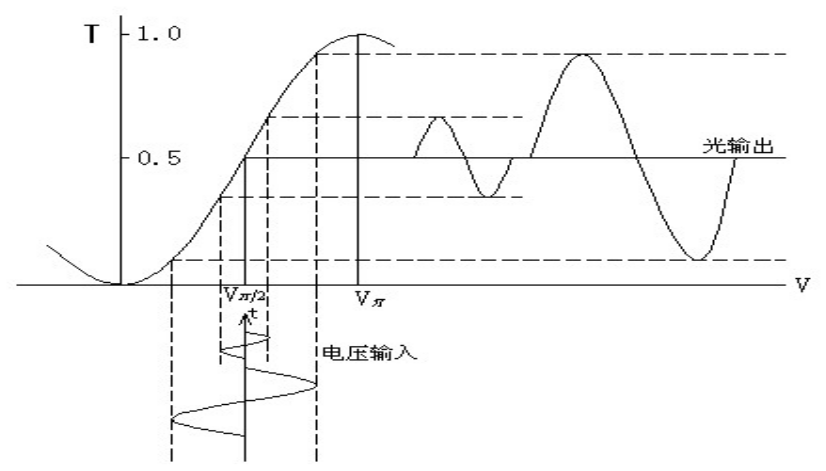
\includegraphics[width=0.7\linewidth]{figures/电光调制原理}
  \caption{电光调制原理图}
\end{figure}

理想的静态工作点是$V_{\pi} / 2$。当$V_0 = V_{\pi} / 2$时,如果有$V_m \ll V_0$,则

\begin{equation*}
  \begin{aligned}
    T \approx \dfrac{1}{2} \left[ 1 + \left( \dfrac{\pi V_m}{V_{\pi}}  \right) \sin \omega t \right]  
  \end{aligned}
\end{equation*}

此时输出波形是我们想要的\textbf{线性调制}信号。

当不满足$V_m \ll V_{\pi}$时,调制信号幅度过大,会出现奇次谐波,输出波形会出现严重\textbf{非线性失真}。

当选择静态工作点$V_0 = \pi$或者$V_0 = 0$时,

\begin{equation*}
  \begin{aligned}
    T \approx \dfrac{1}{8} \left( \dfrac{\pi V_m}{V_\pi}  \right)^2 \left( 1 - \cos 2 \omega t \right) 
  \end{aligned}
\end{equation*}

看上面的原理图很容易明白,由于电压高于静态工作点和低于静态工作点时,输出对称的重复图像,所以输出频率是原先的两倍。这种现象称作\textbf{倍频失真}。

\subsection{依靠改变1/4波片朝向的电光调制}

我们已经知道影响最后投射光强的本质因素是相位差$\delta_1 + \delta_2$(\textbf{依靠改变直流偏压的电光调制}中没有1/4波片,$\delta_2 = 0$),因此我们除了可以调节晶体两端直流偏置电压$V_0$来改变$\delta_1$来改变最终信号光的相位差,也可以通过更改1/4波片的朝向,来改变$\delta_2$,达成相同的目的。

当1/4波片主轴和检偏器光轴夹角为$0$或者$\pi/2$时,$\delta_2 = 0$,和\textbf{依靠改变直流偏压的电光调制}中设置$V_0 = 0$或者$V_0 = V_{\pi}$是一样的,都会输出\textbf{倍频失真}的波形。

当1/4波片主轴和检偏器光轴夹角为$\pi/4$或者$3\pi/4$时,$\delta_2 = \pi/2$,和\textbf{依靠改变直流偏压的电光调制}中设置$V_0 = V_{\pi}/2$是一样的,输出\textbf{线性调制}的波形。

\end{document} 
